\chapter{Introduction Au systeme temps réel}
\minitoc
\section{Introduction}
\section{Taxonomie sur les systèmes temps réel}
\subsection*{Différents niveaux de criticité}

Les systèmes temps réel dits critiques (ou dur) correspondent ont des
systèmes pour lesquelles il est intolérable qu’une échéance soit
manquée au risque de causer des conséquences graves, telles que des
blessures ou des pertes humaines. Les centrales nucléaires ou le
guidage de missiles représentent de tels systèmes à haute
criticité. Dans le domaine de l’informatique embarqué, l’automobile et
l’aéronautique regorgent de systèmes critiques à l’image des
équipements déclencheurs d’airbags ou des logiciels de contrôle de vol
de satellite. Il est crucial que les résultats soient disponibles au
moment voulu et un résultat obtenu trop tard est inutilisable, à
l’instar d’un système anti-missile qui recevrait la position d’un
objet volant avec du retard.

Les systèmes temps réels mou sont des systèmes où on tolère les
retards et ne requièrent pas un déterminisme temporel aussi fort que
les systèmes temps réels dur.  Par exemple, un logiciel de diffusion
de flux vidéo produit un certain nombre d’images dans un intervalle de
temps régulier. Le fait de manquer une ou plusieurs échéances ne
provoque pas l’arrêt du système multimédia. La qualité de la vidéo est
dégradée mais le service peut continuer de fonctionner sans
risque. Donc les systèmes temps réels mou offre le meilleur service
possible (notion de best effort) et les retards dans l’obtention des
résultats ne sont pas dramatiques.

A la frontière entre les systèmes temps réel dur et mou, les systèmes
temps réel ferme tolèrent une certaine proportion d’échéances
manquées. Ils ne considèrent que les résultats obtenus à temps et sont
liés à la notion de qualité de service (QoS).

\section{Modélisation des tâches}
Liu et Layland \cite{LL73} ont proposé une modelisation d'un systemes
temps réel Soit un système temps réel composé d’un ensemble de tâches
nommé $\taskset{}$ qui comprend n tâches périodiques dont les
caractéristiques sont détaillées ci-dessous. Nous définissons dans
cette section tous les termes qui seront utilisés en relation avec la
notion d’ensemble de tâches.
\begin{description}
\item[Tâche :] Une tâche $\task{}$ est définie comme l’exécution
  d’une suite d’instructions. Nous supposons que toutes les tâches
  sont indépendantes et que l’ordre dans lequel les tâches sont
  exécutées n’a pas de conséquence sur la bonne exécution du système
  du moment qu’elles respectent leurs contraintes temporelles. Nous
  faisons également l’hypothèse que les tâches sont synchrones, donc
  que toutes les tâches sont actives dès que le système débute son
  exécution, les tâches sont toutes libérées simultanément. Le modèle
  de tâches que nous utilisons est le modèle de tâches dit périodique
  pour l’ordonnancement fixe et sporadique pour l’ordonnancement
  dynamique.
\item[Travail (Job) :] Chaque tâche libère périodiquement des
  travaux. Un travail est une suite d’instructions qui doit être
  réalisée avant une date fixée. Lorsqu’une tâche libère un travail,
  celui-ci est prêt à être exécuté et devient disponible pour
  l’algorithme d’ordonnancement. Une tâche $\task{i}$ libère ses travaux
  périodiquement suivant sa période Ti, un travail n’a donc pas de
  période associée. Ce modèle est appelé modèle de tâche périodique
  car chaque travail est libéré exactement lorsque la tâche atteint sa
  période. D’autres modélisations plus souples existent comme les
  systèmes de tâches sporadiques ou apériodiques. Pour les systèmes
  sporadiques, la période d’une tâche est la période de temps minimale
  entre deux libérations de travaux pour une tâche, ce qui signifie
  que le système ne peut savoir la date exacte où le travail va être
  libéré. Dans le cas de systèmes apériodiques, l’intervalle de temps
  entre deux libérations de travaux n’est soumis à aucune
  contrainte. Ces systèmes sont plus difficiles à étudier du fait de
  l’imprévisibilité de l’arrivée des tâches.
\item[Hyperpériode :] L’hyperpériode H de l’ensemble de tâches
  correspond au plus petit commun multiple de toutes les périodes de
  l’ensemble de tâches.  $H =
  PPCM(\{\period{0},\period{1},\cdots,\period{n}\})$ Le nombre de
  tâches dans un système temps réel embarqué est limité et les
  périodes de ces tâches ont en général des relations temporelles
  entre elles. Par exemple, il est peu probable que les périodes des
  tâches soient premières entre elles, les périodes des tâches sont
  souvent des harmoniques. En prenant un exemple concret, des tâches
  peuvent avoir des périodes de 1ms, 2ms, 5ms ou 10ms mais il est
  moins fréquent de trouver des tâches avec des périodes de 1.78ms et
  de 8.54ms. La valeur de l’hyperpériode ainsi que le nombre de
  travaux dans une hyperpériode restent donc naturellement
  raisonnables.
\item[Date Réveil :] notée $r_i$, c’est la date où la tache libère
  son premier travail, chaque travail de la tâche est libéré à
  l’instant $r_{i} + K\period{i}~avec~K \in \mathbb{N}$
\item[Pire temps d’execution (Worst Case Execution Time WCET) :] est
  la durée maximale de l’exécution de chacun de ses travaux. Le WCET
  de la tâche $\task{i}$ est noté Ci. Calculer le WCET d’une tâche est
  difficile et ce sujet est une thématique de recherche à lui tout
  seul. Nous renvoyons le lecteur à \cite{WEE+08} pour plus
  d’informations. Nous supposons que le WCET de chaque travail est
  connu.
\item[Échéance(Deadline):] Chaque travail une fois libéré doit
  terminer son exécution avec une certaine date sous peine de violer
  son échéance. Nous notons
  Di l’échéance relative de la tâche

  $\task{i}$. L’échéance absolue $j.d$ du travail $j$ sera donc la
  date de sa libération additionnée de cette échéance relative.

Il existe trois types de modèles  de taches : 

\begin{itemize}
\item Modèles à « échéances implicites » où l’échéance de
  chaque travail égale à sa période $\period{i} = \deadline{i}$.
\item Modèles à « échéances contraintes » où l’échéance de
  chaque travail est inférieure ou égale à sa période $\deadline{i} <=
  \period{i}$.
\item le modèle à «échéances arbitraires» ne fixe aucune
  contrainte entre les échéances et les périodes des tâches.
\end{itemize}

\item[Utilisation d’une tâche :] L’utilisation d’une tâche est le
  rapport entre son WCET et sa période. L’utilisation $U_i$ de la
  t\^ache $\task{i}$ est donc
  $\frac{\charge{i}}{\period{i}}$
\item[Utilisation globale de l’ensemble de tâches :] L’utilisation
  globale U de l’ensemble de tâches est la somme de toutes les
  utilisations individuelles des tâches de l’ensemble de tâches :

\begin{equation}
U = \sum_{i=1}^n U_i
\end{equation}

\end{description}

\section{Ordonnancement monoprocesseur}
Un algorithme d’ordonnancement monoprocesseur est chargé
de répartir les tâches sur un processeur : il décide quelle tâche sera
exécutée sur le processeur et pour combien de temps.
\subsection*{Definition}
Nous définissons dans un premier temps les termes
habituels concernant les systèmes temps réel : \\
\begin{description}
\item[Hors-ligne / en-ligne:] Un algorithme d’ordonnancement
  hors-ligne prend la totalité de ses décisions d’ordonnancement avant
  l’exécution du système. Au contraire, un ordonnancement en-ligne
  prend les décisions d’ordonnancement lors de l’exécution
\item[Priorités:] Les algorithmes d’ordonnancement temps réel peuvent
  être classés suivant leur utilisation des priorités pour choisir
  quelle tâche doit être ordonnancée.
\item[Préemptif / non préemptif:] Un algorithme d’ordonnancement
  préemptif est un algorithme d’ordonnancement qui peut arrêter
  l’exécution d’une tâche, i.e. la préempter, à tout moment lors de
  l’exécution. Au contraire, un algorithme d’ordonnancement non
  préemptif ne permet aucune préemption, un travail en cours
  d’exécution ne peut être arrêté.
\item[Ordonnançabilité / Faisabilité:] Un système de tâches est dit
  ordonnançable si un ordonnancement existe permettant de satisfaire
  toutes les contraintes temps réel. Un système de tâches est dit
  faisable s’il existe un algorithme d’ordonnancement permettant
  d’ordonnancer ce système de tâches sans aucune violation
  d’échéances.
\item[Optimalité:] Un algorithme d’ordonnancement est dit optimal s’il
  peut ordonnancer tous les ensembles de tâches ordonnançables par
  d’autres algorithmes d’ordonnancement existants.
\end{description}
\subsection{Algorithme d’ordonnancement à priorité fixe}
\subsubsection{Rate Monotonic \cite{LL73}}
Rate Monotonic est un algorithme à priorité fixe
introduit par Liu et Layland dans \cite{LL73}. Cet algorithme affecte
des priorités aux tâches inversement proportionnel à leur période :
plus leur période est petite, plus la tâche est prioritaire.

Un exemple de système de tâche ordonnancée par Rate
Monotonic est donné table \ref{tab:exempleRM}. La figure
\ref{fig:exempleRM} est une représentation graphique de
l'ordonnancement correspondant.

\begin{table}[h]
\begin{center}
\begin{tabular}{|c|c|c|c|}
 \hline $\task{i}$ & $\charge{i}$ & $\period{i}$ & priorité\\ 
 \hline 1 & 1 & 10 & 3\\ 
 \hline 2 & 1 & 4 & 0\\ 
 \hline 3 & 1 & 5 & 1\\ 
 \hline 4 & 2 & 8 & 2\\ 
 \hline
 \end{tabular}
\end{center}
\caption{ensemble de tache avec priorité affecté par Rate Monotonic} \label{tab:exempleRM}
\end{table}

%\begin{figure}[h]
%\begin{center}
%\begin{RTGrid}[height=4cm, width=12cm, labelsize=8pt, numbersize=6]{4}{13}
%  \multido{\n=0+4}{3}{
%    \TaskArrDead{2}{\n}{4}}
%  \TaskExecution{2}{0}{1}
%  \TaskExecution{2}{4}{5}
%  \TaskExecution{2}{8}{9}
%  \TaskExecution{2}{12}{13}
%  \multido{\n=0+5}{2}{
%    \TaskArrDead{3}{\n}{5}}
%  \TaskExecution{3}{1}{2}
%  \TaskExecution{3}{5}{6}
%  \TaskExecution{3}{10}{11}
%  \multido{\n=0+8}{1}{
%    \TaskArrDead{4}{\n}{8}}
%  \TaskExecution{4}{2}{4}
%  \TaskExecution{4}{9}{10}
%  \TaskExecution{4}{11}{12}
%  \multido{\n=0+10}{1}{
%    \TaskArrDead{1}{\n}{10}}
%  \TaskExecution{1}{6}{7}
%\end{RTGrid}
%\caption{Ordonnancement sous Rate Monotonic} \label{fig:exempleRM}
%\end{center}
%\end{figure}

\begin{theoreme}
Rate Monotonic est optimal pour l'ordonnancement de systèmes de tâches
synchrones, indépendantes et à échéance sur requête en présence de
préemption.
\end{theoreme}

\begin{theoreme}[Condition Suffisante \cite{LL73}].
  Un système temps réel composé de n tâches est ordonnançable par Rate
  Monotonic si :
\begin{equation}
U = \sum_{i=1}^n \frac{\charge{i}}{\period{i}} \leq n ( 2^{\frac{1}{n}}
- 1)
\end{equation}
\end{theoreme}

\subsubsection{Deadline Monotonic \cite{LW82}}
Deadline Monotonic est un algorithme à priorité fixe
introduit par Leung et Whitehead dans \cite{LW82}.

Cet algorithme est proche de celui de Rate Monotonic, à la différence
que les priorités sont maintenant affectées en fonction de l'échéance
relative de chaque tâche au lieu de leur période.

\begin{theoreme}
Cet algorithme est optimal dans le cadre des algorithmes à priorité
fixe pour des systèmes de tâches synchrones à échéance contrainte
lorsque la préemption est autorisée. Monotonic et Deadline Monotonic
se confondent.
\end{theoreme}

\textbf{Condition suffisante d'ordonnançabilité} La condition
suffisante d'ordonnançabilité est inspirée de la condition suffisante
d'ordonnançabilité de Liu et Layland (cf. théorème 4) :

\begin{theoreme}
 Un système temps réel composé de n tâches est ordonnançable par Deadline
Monotonic si la condition suivante est vérifiée :
\begin{equation}
U = \sum_{i=1}^n \frac{\charge{i}}{\deadline{i}} \leq n ( 2^{\frac{1}{n}} - 1)
\end{equation}
\end{theoreme}

\textbf{Condition necessaire et suffisante d'ordonnançabilité} Joseph
et al. \cite{JP86} ont proposé un test d’ordonnancabilité basé sur le
pire temps de reponse $R_{i}$.  Le pire temps de réponse est le moment
ou la tache $i$ de priorité $p$ terminera son exécution quand les
taches les plus prioritaire sont actifs avec elle en même temps.\\

\begin{theoreme}
soit $\taskset{}$ = \{ $\task{1},\task{2},\cdots, \task{n} \}$ un ensemble de $n$
taches.  $\taskset{}$ est ordonnancable sous deadline monotonic si et seulement si:
\begin{equation}
\forall \task{i} \in \taskset / R_{i} \leq \deadline{i}
\end{equation}

%\begin{equation}
%R_{i} = \left\lbrace
%\begin{array}{l}
%R_{i}^0=\wcet{i}
%\\
% R_{i}^{(k+1)}=\charge{i}+\sum_{j \in pr(i)}  \left \lceil 
% \frac{R_{i}^{(k)}}{\period{j}} \right \rceil * \wcet{j}  
%\end{array}
%\right.
%\end{equation}
\end{theoreme}

\begin{table}[h]
\begin{center}
\begin{tabular}{|c|c|c|c|c|c|}
 \hline$\task{i}$ & $\charge{i}$ & $\deadline{i}$ & $\period{i}$ & $\pr{i}$ & $R_i$\\ 
 \hline1 & 1 & 5 & 10 & 2 & 3\\ 
 \hline2 & 1 & 3 & 4 & 0 & 1\\ 
 \hline3 & 1 & 4 & 5 & 1 & 2\\ 
 \hline4 & 2 & 7 & 8 & 3 & 7\\ 
 \hline
 \end{tabular}
\end{center}
\caption{ensemble de tache avec priorité affecté par Deadline
  Monotonic} \label{tab:exempleDM}
\end{table}


%\begin{figure}[h]
%\begin{center}
%\begin{RTGrid}[height=4cm,width=12cm,labelsize=8pt,numbersize=6]{4}{10}
%\multido{\n=0+10}{1}{
%\TaskArrDead{1}{\n}{5}}
%\TaskExecution{1}{2}{3}

%\multido{\n=0+4}{2}{
%\TaskArrDead{2}{\n}{3}}
%\TaskExecution{2}{0}{1}
%\TaskExecution{2}{4}{5}
%\TaskExecution{2}{8}{9}

%\multido{\n=0+5}{2}{
%\TaskArrDead{3}{\n}{4}}
%\TaskExecution{3}{1}{2}
%\TaskExecution{3}{5}{6}

%\multido{\n=0+8}{1}{
%\TaskArrDead{4}{\n}{7}}
%\TaskExecution{4}{3}{4}
%\TaskExecution{4}{6}{7}
%\end{RTGrid}
%\caption{Ordonnancement sous Deadline Monotonic} \label{fig:exempleDM}
%\end{center}
%\end{figure}


\subsection{Algorithme d’ordonnancement à priorité dynamique}
Les algorithmes à priorité dynamique affectent une priorité qui n'est
plus une donnée statique.  La priorité d'une tâche est mise à jour
durant la vie du système en fonction de certains critères, les
critères utilisés dépendant de l'algorithme utilisé.

\subsubsection{Earliest Deadline First\cite{LL73}}
Earliest Deadline First est un algorithme connu et étudié depuis
longtemps \cite{LL73, Der74, Hor74}. Le principe de cet algorithme est
d'accorder la priorité la plus grande à la tâche ayant une instance
dont l'échéance absolue est la plus proche.  L'avantage majeur de cet
algorithme est qu'en présence d'un système de tâche à échéance sur
requête, le taux d'utilisation maximum du processeur est de 100\%
(théorème 8).

\begin{theoreme}[\cite{LL73}]
 Un système de n tâches à échéance contrainte est ordonnançable par
 Earliest Deadline First si et seulement si :
 \begin{equation}
 U \leq 1
 \end{equation}
\end{theoreme}

\paragraph{Fonction de demande du processeur}

La demande du processeur des tâches devant se terminer avant la date t
(c’est-à-dire dont l’échéance est avant ou à la date t), notée
dbf($\taskset{}$, t) (Demand Bound Function) est définie par la durée
cumulée des requêtes dont la date d’activation et l’échéance sont dans
l’intervalle de temps[0, t]:

\begin{equation}
DBF(\taskset{},t) = \sum_{\task{} \in \taskset{}}dbf(\task{},t)
\end{equation}
%
%\begin{equation}
%dbf(\task{},t) = max \bigg( 0,\bigg( \bigg\lfloor \frac{t - \deadline{i}}{\period{i}} \bigg\rfloor + 1 \bigg) \times \wcet{i} \bigg)
%\end{equation}

\paragraph{Condition necessaire et suffisante
  d'ordonnançabilité}\cite{BHR93} il existe un test d’ordonnancabilité
basée sur la fonction de la demande processeur DBF($\taskset,t$)
causée par des tâches activées et devant être terminées dans
l’intervalle [0, t].

\begin{theoreme}
Un système $\taskset{}$ de $n$ tâches à échéance contrainte est
ordonnançable par Earliest Deadline First si et seulement si :
\begin{equation}
\forall t \geq 0 , DBF(\taskset,t) \leq t 
\end{equation}
\end{theoreme}

\begin{theoreme}[\cite{Der74}]
Earliest Deadline First est optimal pour ordonnancer des systèmes de
tâches indépendantes lorsque le facteur d'utilisation U du système est
inférieur ou égale à 1 (absence de surcharge).
\end{theoreme}

\begin{table}[h]
\begin{center}
\begin{tabular}{|c|c|c|c|}
 \hline$\task{i}$ & $\charge{i}$ & $\deadline{i}$ & $\period{i}$\\ 
 \hline1 & 3 & 4 & 5\\ 
 \hline2 & 3 & 7 & 7 \\  
 \hline
 \end{tabular}
\end{center}
\caption{ensemble de tache } \label{tab:exempleEDF}
\end{table}


%\begin{figure}[h]
%\begin{center}
%\begin{RTGrid}[height=4cm,width=12cm,labelsize=8pt,numbersize=6]{2}{16}
%\multido{\n=0+5}{3}{
%\TaskArrDead{1}{\n}{4}}
%\TaskExecution{1}{0}{3}
%\TaskExecution{1}{6}{9}
%\TaskExecution{1}{12}{15}


%\multido{\n=0+7}{2}{
%\TaskArrDead{2}{\n}{7}}
%\TaskExecution{2}{3}{6}
%\TaskExecution{2}{9}{12}


%\end{RTGrid}
%\caption{Ordonnancement sous EDF} \label{fig:exempleEDF}
%\end{center}
%\end{figure}

\section{Ordonnancement Multiprocesseur}
L'ordonnancement multiprocesseur se distingue de l'ordonnancement
monoprocesseur par la présence de plusieurs processeurs sur lesquels
peuvent s'exécuter les tâches. Se pose alors certains problèmes parmis
eux :
\begin{itemize}
\item[$\bullet$] le problème de placement des tâches : sur quel(s) processeur(s) une tâche va-t-elle s'exécuter ?
\item[$\bullet$] le problème de la migration des tâches : une tâche peut-elle changer de processeur pour s'exécuter ?
\item[$\bullet$] le problème de l'ordonnancement des tâches : affectation des priorités.
\end{itemize}

Nous allons nous intéressé uniquement au problème de placement et
d'ordonnancement des tâches, sans prendre en compte la migration et
nous supposerons que les tâches sont indépendantes.

\subsection{Classification}
 Les algorithmes d'ordonnancement peuvent être classés
dans différentes catégories, en fonction de leurs caractéristiques :
\begin{itemize}
\item  stratégie globale : sur un système comprenant m
  processeurs, un algorithme d'ordonnancement utilisant une stratégie
  globale va affecter les m tâches les plus prioritaires aux m
  processeurs.
\item  stratégie partitionner : le principe d'un algorithme
  utilisant une stratégie par partitionnement est de placer chaque
  tâche sur un processeur, et ensuite d'exécuter sur chaque processeur
  un algorithme d'ordonnancement monoprocesseur.
\item stratégie par semi partitionner : Elle est obtenue
  par combinaison de la stratégie par partitionnement et de la
  stratégie globale.
\end{itemize}
Il est à noter qu'il n'y a pas une catégorie qui soit
meilleure qu'une autre. Il existe des systèmes de tâches qui peuvent
être ordonnancés en utilisant une stratégie globale mais pas avec une
stratégie par partitionnement et inversement. On dit que ces
algorithmes sont non comparables \cite{LW82}.

\subsection{Optimalité}
\begin{theoreme}[\cite{HL92}]
Il n'existe pas d'algorithme en-ligne optimal pour des systèmes
multiprocesseurs. Toutefois, lorsqu'on restreint le cadre d'étude et
que l'on ne considère uniquement des systèmes de tâches périodiques,
alors il existe des algorithmes optimaux, comme les algorithmes de
type Pfair par exemple.
\end{theoreme}

\subsection{Algorithme d'ordonnancement utilisant une stratégie par partitionnement}
\subsubsection{Généralité}
Les algorithmes utilisant une stratégie par
partitionnement relèvent dans la plupart des cas du problème du
bin-packing, c'est-à-dire comment trouver un placement pour l'ensemble
des tâches sur un nombre minimum de processeurs.  Ce problème de
partitionnement des tâches pour les placer sur les processeurs a été
montré comme étant NP-difficile dans \cite{LW82}. Il n'existe donc pas
d'algorithmes s'exécutant en temps polynomial permettant de trouver
une solution optimale à ce problème. Toutefois, il existe des
heuristiques permettant d'obtenir des résultats corrects en temps
polynomial.
\subsubsection{First-Fit et Best-Fit}
Parmi les heuristiques existantes pour résoudre ce type de problème,
il existe quatre heuristiques First Fit, Best Fit, Next Fit et Worst
Fit qui reposent tous sur le même principe : on affecte chaque tâche
dans l'ordre à un processeur, selon un critère d'acceptation.  La
différence entre les deux types d'algorithmes réside sur la manière
dont est placée chaque tâche :
\begin{itemize}
\item[$\bullet$] First Fit : la tâche est placée sur le premier
  processeur avec un ensemble de tache ordonnançable ;
\item[$\bullet$] Next Fit : même principe que First Fit ...
\item[$\bullet$] Best Fit : la tâche est placée sur le processeur avec
  un ensemble de tache ordonnançable et ayant le taux d'utilisation
  maximal.
\item[$\bullet$] Worst Fit : la tâche est placée sur le processeur
  avec un ensemble de tache ordonnançable et ayant le taux
  d'utilisation minimal.
\end{itemize}
Les algorithmes de type First Fit ou Best Fit ne sont pas les seuls
existants il existe aussi Next Fit ou aussi Worst Fit.

La table \ref{tab:exampleFFBF} et les figures \ref{fig:exemplFF} et
\ref{fig:exemplBF} illustre les deux heuristiques de placement
First-Fit et Best-Fit sur un ensemble de 10 taches periodiques et 4
processeurs.

\begin{table}[!h]
\begin{center}
\begin{tabular}{|c|c|c|c|}
 \hline$\task{i}$ & $\charge{i}$ & $\deadline{i}$ & $\period{i}$ \\ 
 \hline1 & 5 & 10 & 10 \\ 
 \hline 2 & 7 & 21 & 21 \\ 
 \hline 3 & 3 & 22 & 22 \\ 
 \hline 4 & 1 & 24 & 24 \\ 
 \hline 5 & 10 & 30 & 30 \\ 
 \hline 6 & 16 & 40 & 40 \\ 
 \hline 7 & 1 & 50 & 50 \\ 
 \hline 8 & 3 & 55 & 55 \\ 
 \hline 9 & 9 & 70 & 70 \\ 
 \hline 10 & 17 & 100 & 100 \\ 
 \hline 
 \end{tabular}
\end{center}
\caption{Ensemble de taches periodiques} \label{tab:exampleFFBF}
\end{table}

\begin{figure}[!h]
\begin{center}
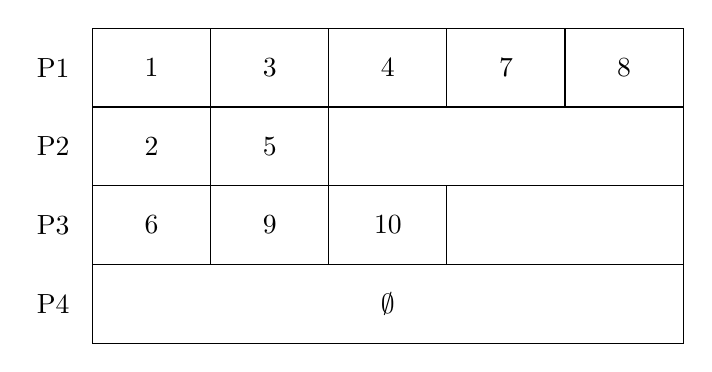
\begin{tikzpicture}
%\draw (0,0) rectangle (1.5,1);
\node at (-0.5,0.5) {P4};
\node at (-0.5,1.5) {P3};
\node at (-0.5,2.5) {P2};
\node at (-0.5,3.5) {P1};
\draw (0,1) rectangle (1.5,2) node[pos=.5] {$\task{6}$};
\draw (0,2) rectangle (1.5,3) node[pos=.5] {$\task{2}$};
\draw (0,3) rectangle (1.5,4) node[pos=.5] {$\task{1}$};
\draw (1.5,1) rectangle (3,2) node[pos=.5] {$\task{9}$};
\draw (1.5,2) rectangle (3,3) node[pos=.5] {$\task{5}$};
\draw (1.5,3) rectangle (3,4) node[pos=.5] {$\task{3}$};
\draw (3,1) rectangle (4.5,2) node[pos=.5] {$\task{10}$};
\draw (3,3) rectangle (4.5,4) node[pos=.5] {$\task{4}$};
\draw (4.5,3) rectangle (6,4) node[pos=.5] {$\task{7}$};
\draw (6,3) rectangle (7.5,4) node[pos=.5] {$\task{8}$};
\draw (0,0) rectangle (7.5,4);
\draw (0,0) rectangle (7.5,4);
\draw (0,0) rectangle (7.5,3);
\draw (0,0) rectangle (7.5,2);
\draw (0,0) rectangle (7.5,1) node[pos=.5] {$\emptyset$};
\end{tikzpicture}
\caption{Placement de taches en First Fit par les contraintes
  DM} \label{fig:exempleFF}
\end{center}
\end{figure}

\begin{figure}[!h]
\begin{center}
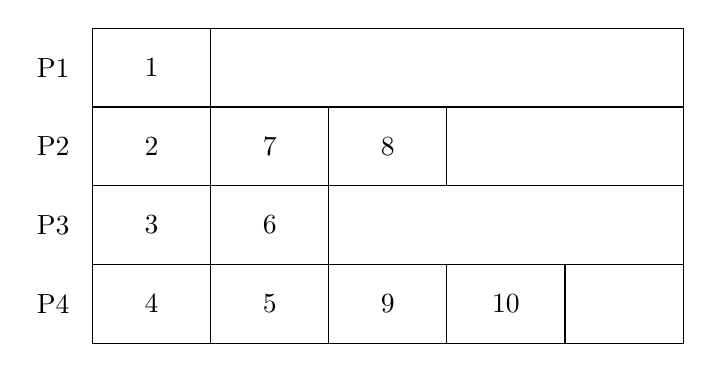
\begin{tikzpicture}
\node at (-0.5,0.5) {P4};
\node at (-0.5,1.5) {P3};
\node at (-0.5,2.5) {P2};
\node at (-0.5,3.5) {P1};
\draw (0,0) rectangle (1.5,1) node[pos=.5] {$\task{4}$};
\draw (0,1) rectangle (1.5,2) node[pos=.5] {$\task{3}$};
\draw (0,2) rectangle (1.5,3) node[pos=.5] {$\task{2}$};
\draw (0,3) rectangle (1.5,4) node[pos=.5] {$\task{1}$};

\draw (1.5,0) rectangle (3,1) node[pos=.5] {$\task{5}$};
\draw (1.5,1) rectangle (3,2) node[pos=.5] {$\task{6}$};
\draw (1.5,2) rectangle (3,3) node[pos=.5] {$\task{7}$};

\draw (3,0) rectangle (4.5,1) node[pos=.5] {$\task{9}$};
\draw (3,2) rectangle (4.5,3) node[pos=.5] {$\task{8}$};

\draw (4.5,0) rectangle (6,1) node[pos=.5] {$\task{10}$};
\draw (0,0) rectangle (7.5,4);
\draw (0,0) rectangle (7.5,4);
\draw (0,0) rectangle (7.5,3);
\draw (0,0) rectangle (7.5,2);
\draw (0,0) rectangle (7.5,1);
\end{tikzpicture}
\caption{Placement de taches en Best Fit par les contraintes
  DM} \label{fig:exempleBF}
\end{center}
\end{figure}
\section{Conclusion}
